\section{The proposed ROI fusion pipeline}\label{sec:pipeline}
AVF combines the probabilities of a tree and a jointly balanced neural model trained on the same regional inputs (Figure~\ref{fig:pipeline}). Alternative losses and neural fusion members serve as controls.
\begin{figure}[pos=!ht]
\centering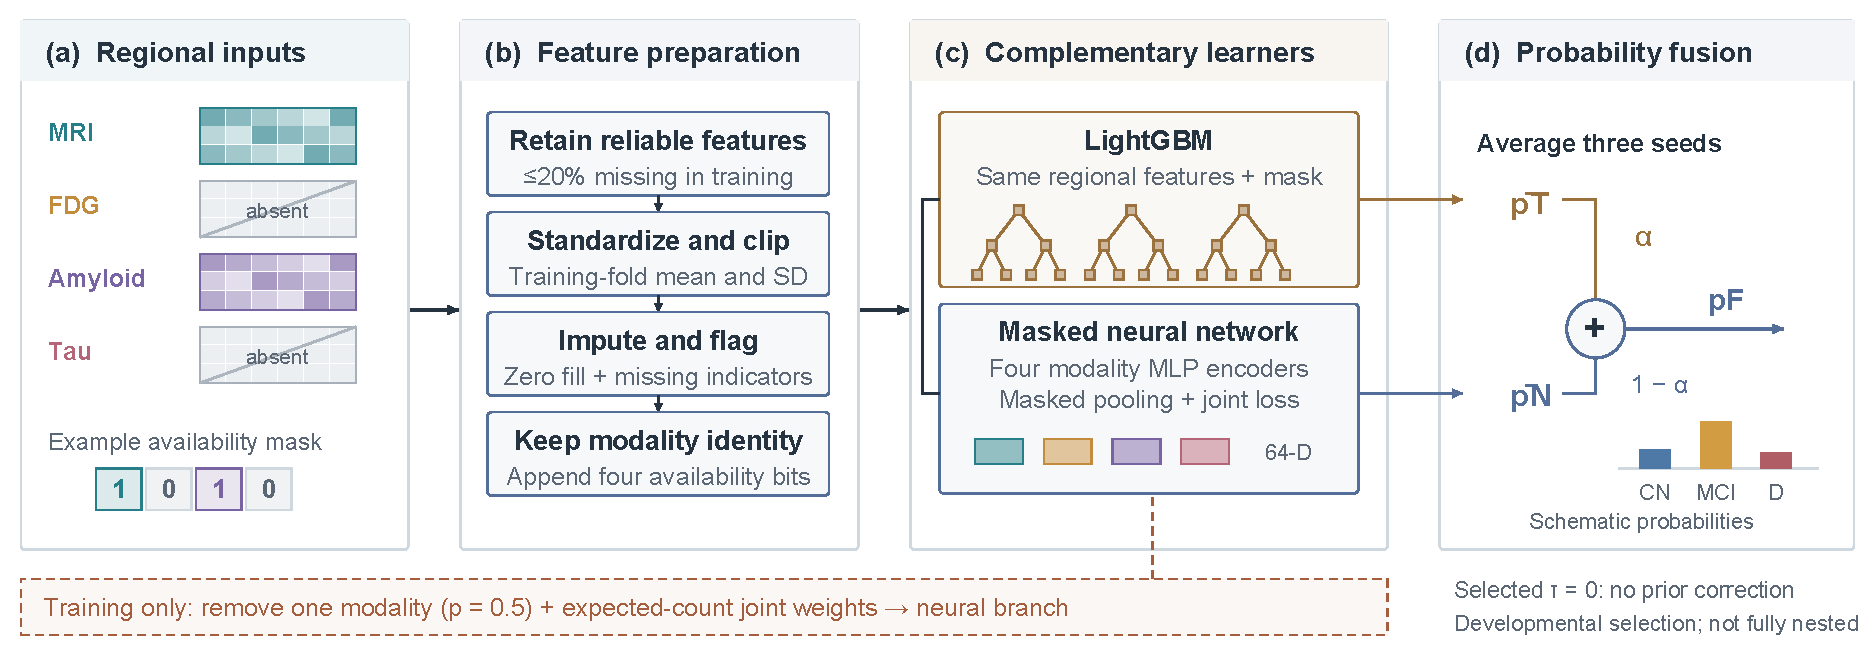
\includegraphics[width=\linewidth]{roi_pipeline}
\caption{AVF overview: regional inputs, training-fold preparation, complementary learners and probability fusion. Dashed links denote neural training controls. Tiles and output bars are schematic. Selection is developmental, not fully nested.}\label{fig:pipeline}
\end{figure}

\subsection{Complementary prediction branches}
\paragraph{Tree branch.} LightGBM receives concatenated regional blocks, feature-missing flags and four availability bits. It is trained without the neural cell-weighting objective. The reference and the fusion use the mean probabilities of the same three tree training seeds.

\paragraph{Neural branch.} Each modality has an MLP encoder producing $h_k\in\mathbb{R}^{64}$. It comprises linear, GELU and LayerNorm transformations with hidden dropout 0.1. A learned scalar gate $g$ defines masked pooling:
\begin{equation}
a_k=\frac{m_k\exp(g(h_k))}{\sum_j m_j\exp(g(h_j))},\qquad
h=\sum_k a_kh_k,\qquad z=f_{\theta}([h;m]).
\end{equation}
The implementation assigns absent gate scores $-10^9$ before softmax. The head maps the 68-value concatenation of the pooled token and mask to three logits. Softmax produces diagnosis probabilities. Figure~\ref{fig:architecture} expands feature preparation, modality encoders and masked pooling. The mask is a predictive input, so attention pooling should not be interpreted as eliminating missingness shortcuts.
\begin{figure}[pos=!ht]
\centering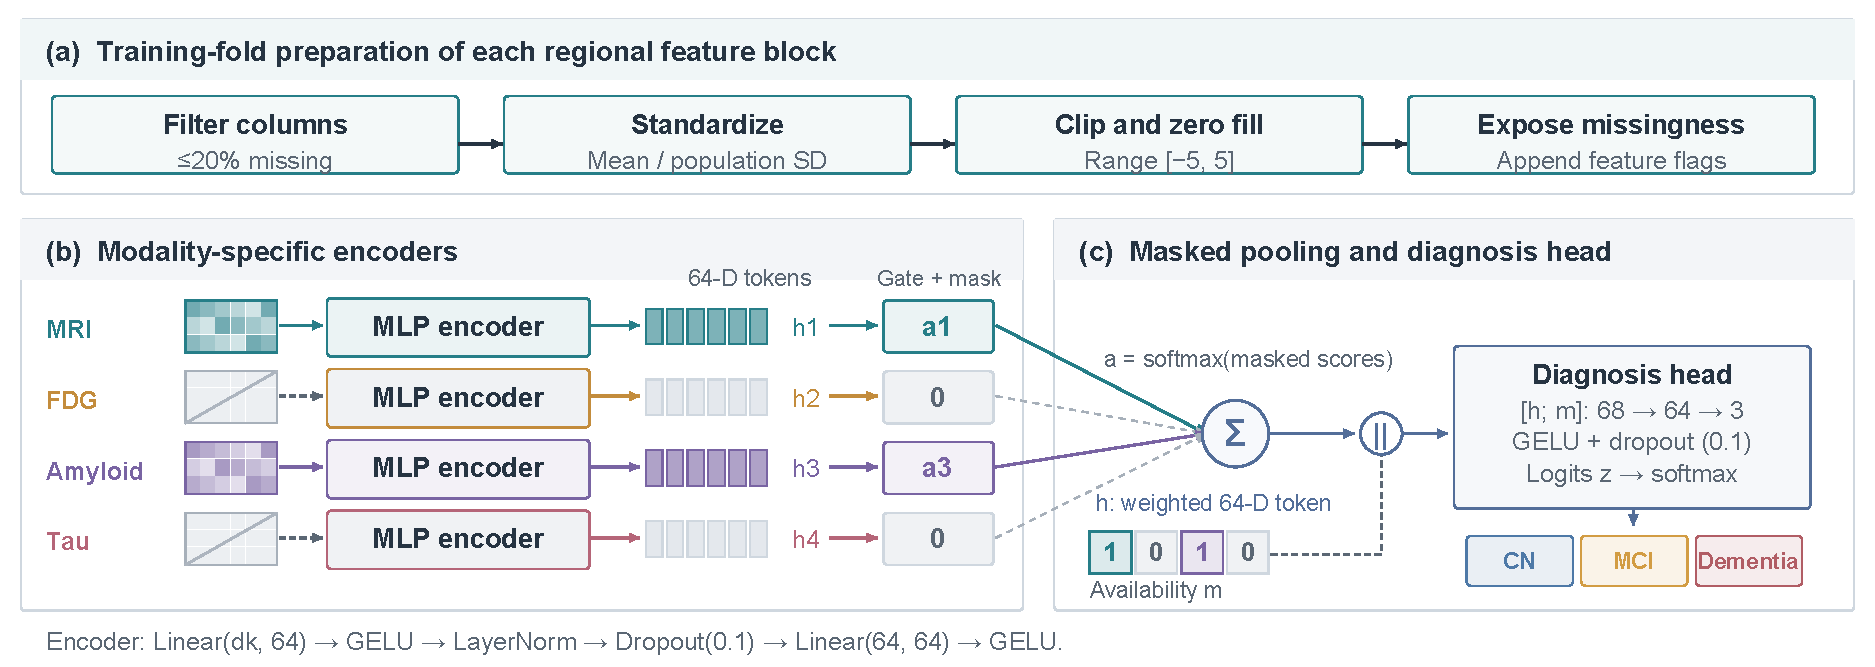
\includegraphics[width=\linewidth]{roi_architecture}
\caption{Neural branch: (a) feature preparation, (b) modality MLPs and 64-dimensional tokens, (c) masked pooling and diagnosis head. Grey tokens are excluded from pooling; encoder outputs need not be zero. The mask is illustrative.}\label{fig:architecture}
\end{figure}

\subsection{Modality dropout and joint weighting}
For episodes with at least two available modalities, training removes one uniformly chosen modality with probability 0.5 and updates its mask. Singleton episodes retain their modality. If $D(p)$ is the set of one-modality descendants of $p$ and $k(p)$ its number of modalities, expected effective counts are
\begin{equation}
E_{q,c}=\sum_p n_{p,c}T(q\mid p),\quad
T(q\mid p)=\begin{cases}
1 & k(p)=1,\ q=p,\\
1/2 & k(p)>1,\ q=p,\\
1/(2k(p)) & k(p)>1,\ q\in D(p),\\
0 & \text{otherwise}.
\end{cases}
\end{equation}
Thus 100 examples with MRI and FDG contribute expected masses 50 to the original pattern and 25 to each singleton descendant. Figure~\ref{fig:weighting} relates observed imbalance to this redistribution.
\begin{equation}
\widetilde w_{q,c}=\operatorname{clip}\!\left(\sqrt{\frac{N}{45(E_{q,c}+5)}},0.25,4\right),\qquad
w_{q,c}=\frac{\widetilde w_{q,c}}{N^{-1}\sum_{r,d}E_{r,d}\widetilde w_{r,d}}.
\end{equation}
The additive five smooths sparse counts; clipping occurs before mean-one normalization. Consequently, the final weights need not remain within the clipping bounds. The neural objective averages $w_{q_i,c_i}\operatorname{CE}(z_i,c_i)$ over a batch. No-dropout joint weighting substitutes natural counts for $E$. Class weighting uses an analogous three-class formula. These rules change influence rather than generating independent subjects.
\begin{figure}[pos=!ht]
\centering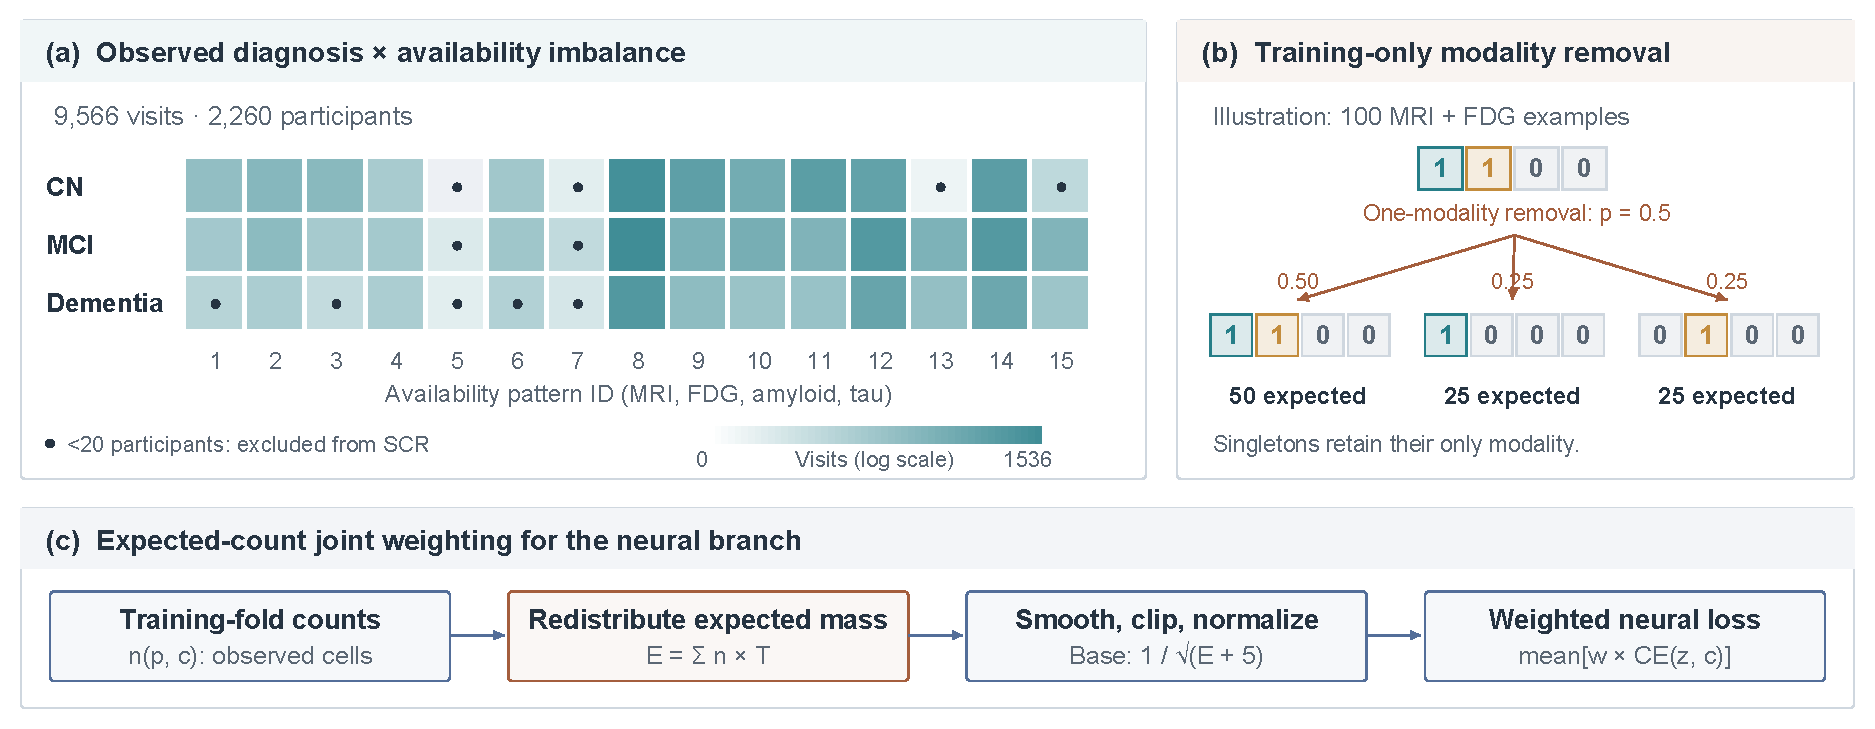
\includegraphics[width=\linewidth]{roi_joint_weighting}
\caption{Joint imbalance: (a) descriptive cohort counts; dots mark unsupported SCR cells, (b) illustrative dropout redistribution, (c) weighting from training-fold expected counts. Full-cohort counts are descriptive only.}\label{fig:weighting}
\end{figure}

\subsection{Probability fusion and its selection}
Let $\bar p^{T}$ and $\bar p^{N}$ denote probabilities averaged over three seeds for the tree and neural branches. AVF forms
\begin{equation}
p^{F}=\alpha\bar p^{T}+(1-\alpha)\bar p^{N}.
\end{equation}
For $\tau>0$, the archived search also allowed an optional prior correction,
\begin{equation}
p^{A}=\operatorname{softmax}\{\log\operatorname{clip}(p^{F},10^{-12},1)
+\tau[\log(1/3)-\log\operatorname{clip}(\bar P(c\mid p),10^{-6},1)]\},
\end{equation}
where $\bar P(c\mid p)=(n_{p,c}+20P(c))/(n_p+20)$ and $P(c)$ is the training-fold class frequency. Tuning averages the prior matrices of the other folds; application uses the target fold's training prior. At $\tau=0$, the implementation returns $p^F$ directly. The grid used $\alpha=0,0.05,\ldots,1$ and $\tau\in\{0,0.25,0.5,0.75,1,1.5\}$. It maximized natural macro-F1 on predictions from the other two folds, then applied the choice to the target fold. Selected tree weights were 0.55, 0.60 and 0.55; every selected $\tau$ was zero. The reported AVF is therefore the probability mixture without an active prior correction.

The leave-one-fold-out fusion search is not fully nested: the models that generate its tuning-fold predictions were trained on subjects from the target fold. Each reported validation fold also selected its own checkpoint epoch. A base learner does not fit its own held-out subjects, but that separation does not remove the selection dependencies. Generalization claims must therefore remain limited.
